\section{Provisorischer Aufbau}
\label{provi}

Der Provisorische Aufbau diente zum Testen der verwendeten Bauteile, sowie dem Erstellen der Musterlösung zugehörig zur Laborübung.

Hier wird der Motor durch eine Zange mit Lederschutz gebremst.
Weiters ist er nur ungenau in zugeschnittenen Rohren gelagert, welche mittels eines angschweißten Bolzens fixiert werden.

Hier traten einige Probleme auf:

\begin{itemize}
    \item Fertigung einer Scheibe zur Drehzahlmessung
    \item Schweißen der dünnen Rohre zur Lagerung des Motors
    \item Schweißen des Armes auf die Rohrschelle
    \item Hohe Hitzeentwicklung beim Bremsen des Motors
\end{itemize}

Der provisorische Aufbau erfüllt alle Anforderungen an den Versuchsaufbau, ist jedoch nicht benutzerfreundlich und liefert nur ungenaue Messungen.

\begin{figure}[H]
    \begin{center}
        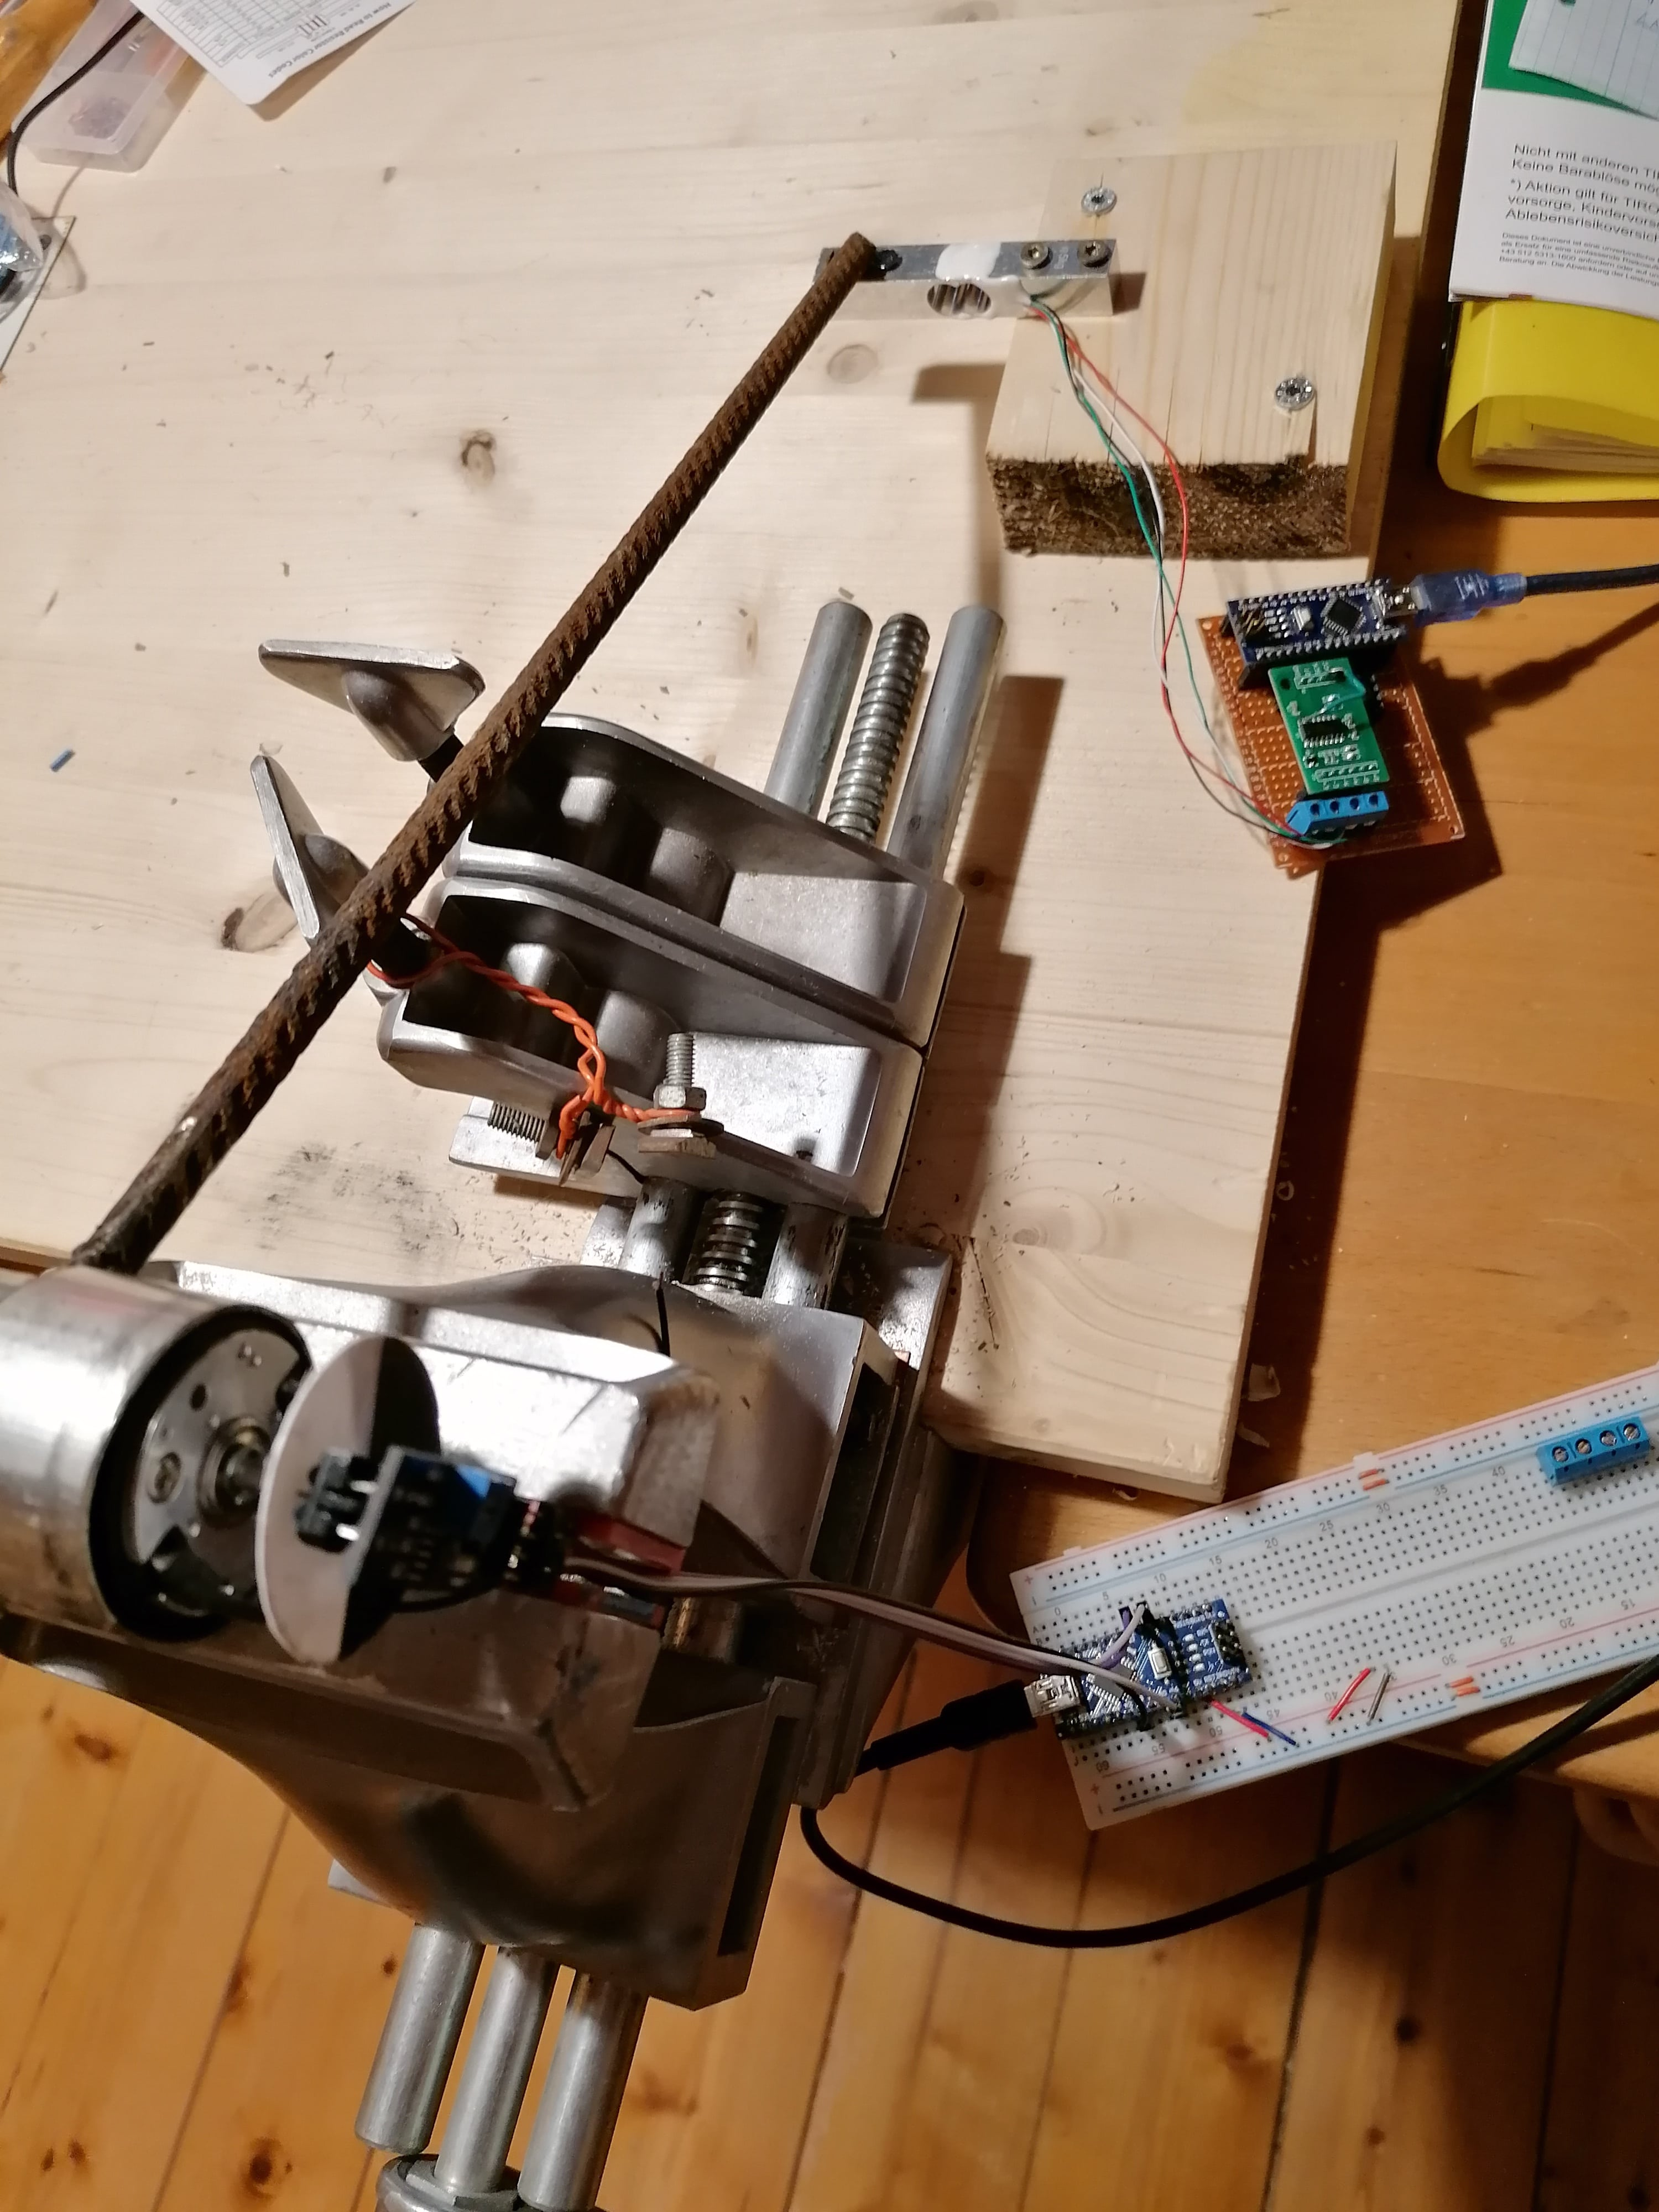
\includegraphics[width=0.3\textwidth]{versuchsaufbau1.jpg}
        \caption{Provisorischer Versuchsaufbau}
    \end{center}
\end{figure}